\documentclass{standalone}
\usepackage{tikz}
\usepackage{newtxmath}
\usetikzlibrary{decorations.markings,decorations.pathmorphing,arrows,positioning,calc}

\begin{document}

\definecolor{newgreen}{RGB}{33,172,47}

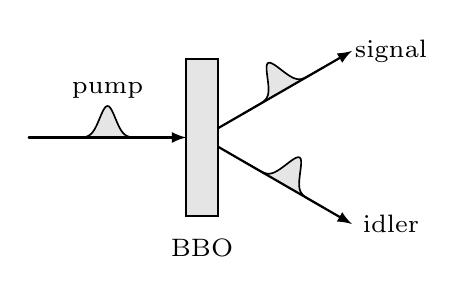
\begin{tikzpicture}[scale=2, every node/.style={scale=1.3},wave/.style={semithick,color=#1,smooth}]
       
    \begin{scope}
    \draw[wave=black, fill=black!10, variable=\x, samples at={-0.3,-0.29,...,0.3}] plot (\x-0.6, {0.2*e^(-\x*\x/0.005)+0.5});
    \draw[thick, -latex, line cap=round] (-1.1,0.5) -- (-0.1, 0.5);
    \node[black] at (-0.6,0.8) {\scriptsize pump};
    \end{scope}

    \begin{scope}[rotate around={30:(0.0,0.5)}]
    \draw[wave=black, fill=black!10, variable=\x, samples at={-0.3,-0.29,...,0.3}] plot (\x+0.6, {0.2*e^(-\x*\x/0.005)+0.5});
    \draw[thick, -latex] (0.0,0.5) -- (1.1,0.5);
    \end{scope}

    \begin{scope}[rotate around={-30:(0.0,0.5)}]
    \draw[wave=black, fill=black!10, variable=\x, samples at={-0.3,-0.29,...,0.3}] plot (\x+0.6, {0.2*e^(-\x*\x/0.005)+0.5});
    \draw[thick, -latex] (0.0,0.5) -- (1.1,0.5);
    \end{scope}
        
    \draw[thick, fill=gray!20] (-0.1,0) rectangle (0.1,1);

    \node[] at (0,-0.2) {\scriptsize BBO};
    \node[] at (1.2,1.05) {\scriptsize signal};
    \node[] at (1.2,-0.05) {\scriptsize idler};
\end{tikzpicture}


\end{document}